\section{Durchführung}
\label{sec:Durchführung}

%Wollen wir noch Abbildungen einfügen?

\subsection{Aufbau}
\label{sec:Aufbau}

Für alle Versuchsteile wird ein Generator mit variablem Schwingungsmuster verwendet. Ein Tiefpassfilter wird an den Generator angeschlossen.
Der Tiefpassfilter wird mit einem Kondensator und einem Widerstand realisiert. Die Kondensatorspannung wird mit einem Oszilloskop gemessen.

\subsection{Messung}
\label{sec:Messung}

\begin{figure}[h!]
    \centering
    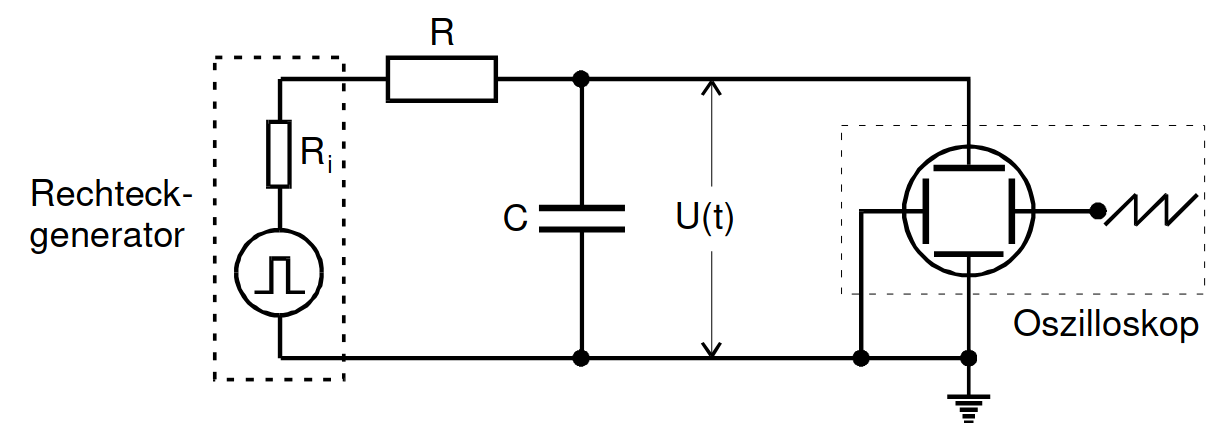
\includegraphics[width=\linewidth]{img/Aufbau1.png}
    \caption{Schematischer Aufbau des ersten Versuchteils\cite{V353}}
    \label{fig:Aufbau1}
\end{figure}

Im ersten Aufgabenteil wird die Zeitkonstante eines RC-Gliedes ermittelt.
Dazu wird eine Rechteckspannung an den Kondensator angeschlossen. Mit dem Oszilloskop wird die Spannung $U_C$ am Kondensator gemessen. %doppelt gemoppelt?
Die Frequenz der Rechteckspannung und der Messbereich des Oszilloskops werden so gewählt, dass ein vollständiger Be- oder Entladevorgang
auf dem Oszilloskop abgebildet werden kann. Es werden Messwertpaare der Form $(t, U_C)$ aufgezeichnet.\\

\begin{figure}[h!]
    \centering
    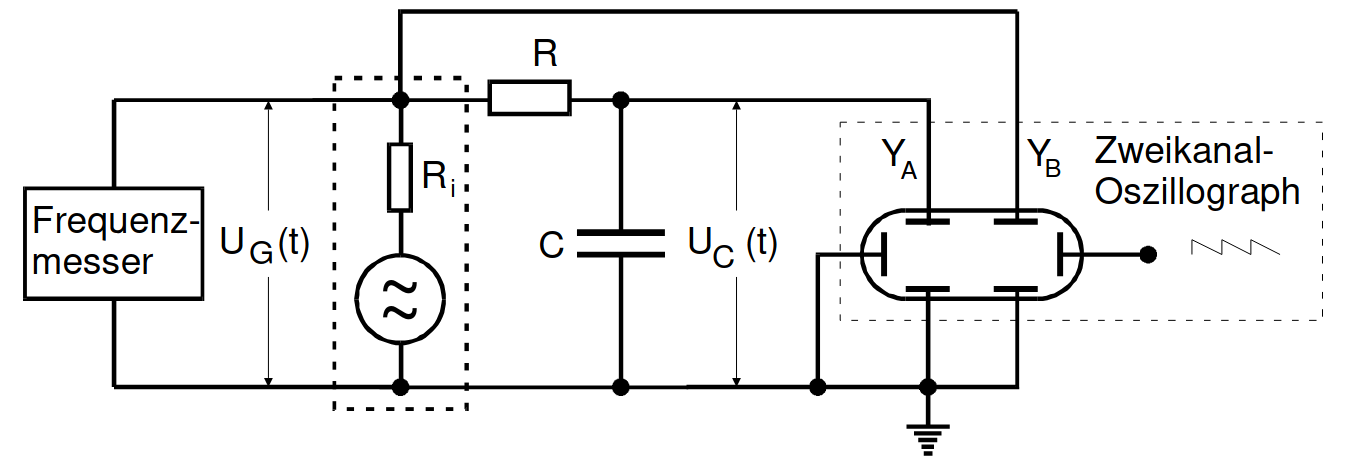
\includegraphics[width=\linewidth]{img/Aufbau2.png}
    \caption{Schematischer Aufbau des zweiten Versuchteils\cite{V353}}
    \label{fig:Aufbau2}
\end{figure}

Im zweiten Aufgabenteil wird die Frequenzabhängigkeit der Kondensatorspannung $U_C$ untersucht. Dazu wird eine Sinusspannung an den Kondensator angeschlossen.
Mit einem Oszilloskop wird die Spannung $U_C(t)$ am Kondensator und die Generatorspannung $U_{\symup{G}}(t)$ gemessen. %Auch überflüssig?
Die Frequenz der Sinusspannung wird von 41.1 Hz bis 1 kHz gesteigert.
Die Generatorspannung und die Kondensatorspannung werden auf dem Oszilloskop gegen die Zeit abgebildet.
Es werden immer vier Messwerte aufgenommen. Die Frequenz $f$, die Generatorspannung $U_{\symup{G}}$, der zeitliche Abstand $a$ der beiden Nulldurchgänge der Schwinungen und die Schwinungsdauer $b$ einer Schwingung werden gemessen.
\\
\\
Für den dritten Aufgabenteil wird die Frequenz des Generators $ω >> \frac{1}{RC}$ gewählt, damit der Tiefpassfilter als Integrator wirkt.
Nacheinander wird eine Dreieck-, Rechteck- und Sinusspannung auf das RC-Glied gegeben. Die Ausgangsspannung und die integrierte Spannung
werden auf dem Bildschirm des Oszilloskops abgebildet. Es werden Bilder für die drei Spannungen aufgenommen.\\
\newpage